\begin{figure}[htp]
\centering

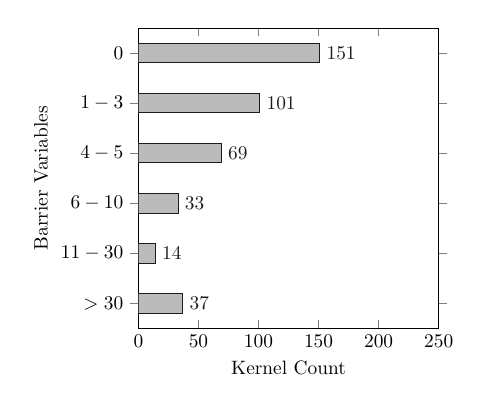
\begin{tikzpicture}[scale=0.7]

\selectcolormodel{gray}

\begin{axis}[
    xbar, xmin=0, xmax=250,
    xlabel={Kernel Count},
    symbolic y coords={
        {$> 30$},
        {$11-30$},
        {$6-10$},
        {$4-5$},
        {$1-3$},
        {$0$}
    },
    ytick=data,
    ylabel={Barrier Variables},
    nodes near coords,
    nodes near coords align={horizontal},
    height=200pt, width=200pt
]

\addplot coordinates {
    (37,{$> 30$})
    (14,{$11-30$})
    (33,{$6-10$})
    (69,{$4-5$})
    (101,{$1-3$})
    (151,{$0$})
};

\end{axis}
\end{tikzpicture}

\caption{Barrier Variables}
\label{Fi:barrier_variables}

\end{figure}
